%Basics
\documentclass[aps, prl, reprint, a4paper, english, 12pt, twocolumn]{revtex4}
\bibliographystyle{apsrev4-1}
\usepackage[utf8]{inputenc}
\usepackage{babel}

%Symbols and scientifics
\usepackage{amsmath}
\usepackage{commath}
\usepackage{amsfonts}
\usepackage{amssymb}
\usepackage{physics}
\usepackage{mathtools}
\usepackage{siunitx}
\sisetup{
per-mode = fraction ,
round-mode = figures ,
round-precision = 3 ,
scientific-notation = engineering ,
output-decimal-marker = {.} ,
exponent-product = \times ,
separate-uncertainty = true ,
uncertainty-separator = \ ,
output-product = \cdot ,
quotient-mode = fraction ,
range-phrase = - ,
range-units =  single ,
inter-unit-product = \ensuremath{{\cdot{}}} ,
number-unit-product = \ ,
multi-part-units = single ,
}
\usepackage{units}

%Appendix, TOC and Bibliography
\usepackage{appendix}
\renewcommand\appendixtocname{Appendices}
%\usepackage[nottoc]{tocbibind}
\usepackage{natbib}
\setcitestyle{numbers,square}
\usepackage[lastpage,user]{zref}

%Figures
\usepackage[svgnames]{xcolor} % Required to specify font color
\usepackage{tikz}
\usetikzlibrary{shadings}
\usepackage{float}
\usepackage{rotating}
\usepackage{graphicx}
\usepackage{wrapfig}
\usepackage[rmargin=2.5cm, tmargin=2.5cm, lmargin=2.5cm, bmargin=2.5cm]{geometry}
\usepackage{xcolor}
\usepackage{etoolbox}
\usepackage{verbatim}
\usepackage[space]{grffile}
\usepackage[final]{pdfpages}
\usepackage{array}
\usepackage{multirow}

%Header footer
\usepackage{fancyhdr}
\pagestyle{fancy}
\lhead{F. G. Kristensen,\\C. V. Sørensen og R. K. F. Wiuff}
\chead{Nanomechanics for graphene membranes\\}
\rhead{10/1-2018\\Course 34029: Physics Project}
\cfoot{Side \thepage\, af \zpageref{LastPage}}
\renewcommand{\headrulewidth}{0.4pt}
\renewcommand{\footrulewidth}{0.4pt}

%Text tools
\usepackage[normalem]{ulem}
\usepackage{import}
\usepackage{newclude}
\usepackage{url}
\usepackage{lipsum}
\usepackage{microtype}
\usepackage{hyperref}
\hypersetup{
  colorlinks   = true, %Colours links instead of ugly boxes
  urlcolor     = blue, %Colour for external hyperlinks
  linkcolor    = blue, %Colour of internal links
  citecolor   = red %Colour of citations
}
\usepackage[capitalise]{cleveref}
\usepackage{enumitem}
\usepackage{booktabs}
\usepackage{silence}
\WarningFilter{revtex4-1}{Repair the float}

%Python
\usepackage{minted}
\usemintedstyle{monokai}
\renewcommand{\listoflistingscaption}{Listings}

%Definitions and new commands
\setlength{\parindent}{0pt}
\setlength{\parskip}{1ex plus 0.5ex minus 0.2ex}
\newcommand{\logas}[1]{\log_{_{10}}{\left( #1 \right)}}
\newcommand{\sins}[1]{\sin{\left( #1 \right)}}
\newcommand{\tans}[1]{\tan{\left( #1 \right)}}
\newcommand{\coss}[1]{\cos{\left( #1 \right)}}
\newcommand{\sinas}[1]{\sin{\left( #1 \degr \right)}}
\newcommand{\tanas}[1]{\tan{\left( #1 \degr\right)}}
\newcommand{\cosas}[1]{\cos{\left( #1 \degr\right)}}
\newcommand{\lnas}[1]{\mathrm{ln}\left( #1 \right)}
\newcommand{\degr}{^{\circ}}
\newcommand{\me}{\mathrm{e}}
\newcommand{\eula}[1]{ \dpd{L }{#1} - \dod{}{t}\left(\dpd{L}{\dot{#1}}\right)}
\begin{document}

%Titlepage herunder:
\begin{abstract}
 \begin{description}
  In this report we will focus on nanomembranes and analyse how this react when a force is applied to them. Nanomembranes can be fabricated via the method of chemical vapor deposition (CVD) and this have been test in the lab by using electrostatic gates \cite{Zande2010}. There are also examples of using lasers to drive a vibration in a membrane \cite{Davidovikj2016} but both of this membranes however are way lager then the ones we will be studying in this report. the concept of carbon nanomembranes have existed for a couple of years all ready so what we are going to focus on are the the smallest nanomembranes that can be made right now.
 \end{description}
\end{abstract}

\title{Nanomechanics for graphene membranes}
\date{10/1-2018}
\author{Frederik Grunnet Kristensen (s164003)}
\email[E-mail at ]{s164003@student.dtu.dk}
\author{Christoffer Vendelbo Sørensen (s163965)}
\email[E-mail at ]{s163965@student.dtu.dk}
\author{Rasmus Kronborg Finnemann Wiuff (s163977)}
\email[E-mail at ]{s163977@student.dtu.dk}
\affiliation{Technical University of Denmark}
\homepage[Homepage of the Technical University of Denmark ]{http://www.dtu.dk/english/}

\maketitle

\pagenumbering{arabic}

\tableofcontents
\thispagestyle{empty}
\newpage
\setcounter{page}{1}

%Text
\section{Introducing the project}
% !TEX root = ../Main.tex

Since the isolation and characterisation of
Graphene in 2004 by Andre Geim and
Konstantin Novoselov, scientists have marvelled over the physical properties and potential
application of Graphene. Being a relatively new material, many aspects and ideas are being
investigated and researched at all times. Graphene yield extreme tensile strength as well as
extreme electric conductivity, yet its structure is fairly simple. Graphene consists solely of
carbon atoms thus making it easy to simulate using specialised software, since carbon atoms are greatly understood in terms of chemical
bonding.
As graphene is a very versatile material the possibilities for research in simulation enviroments are virtually limitless.
Therefore it is basically possible to make experiments limited only by imagination, in order
to discover new properties and possible applications of graphene. This saves resources
before entering the lab, where the simulated reality is tested.

In this rapport we will simulate and analyse the properties of nanomembranes as done in the papir "Visualizing the Motion of Graphene Nanodrums"\cite{Davidovikj2016}, which Figure \cref{Motivation} stems from. It shows how phonos travel through this membranes. However there this article,as many others, focuses on membranes in the micro-scale we will examine if this same phenomenons are found at the nano-scale. To do this we start by considering at ideal system of just one sheet of carbon atoms.
To make a more praticel membrane we will investigate if you can create the same membrane effects if you take a graphene layer and put it on top of a substrate with different sized and shaped holes, to form
form this nanomembrane and this is the that we will be looking at. It is expected possible to create such a nanomembrane at the
size of few tens of nanometers at Nanotech with Block-copolymer lithography or TEM
structuring of a substrate. In a virtual environment, it is possible to simulate phonons
in the graphene atop of these holes in the membrane. The purpose of this project is to
simulate phonons in the nanomembrane and find the optimal conditions for producing
phonons in the terahertz spectrum.
We will employ the software Atomistic ToolKit (ATK) to calculate phonon properties
of membranes as well as performing molecular dynamics of the excited membrane. The
software will enable prompt setup of relevant structures so that more time is free to analysis
and actual simulations.
\begin{figure}
    \centering
    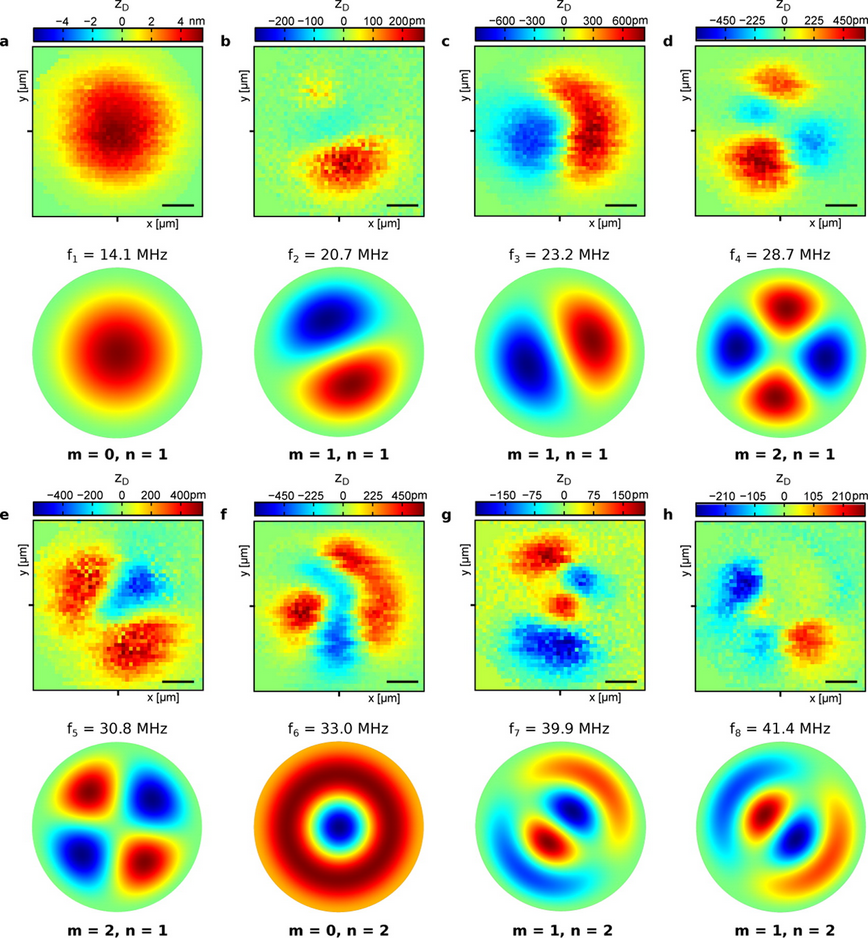
\includegraphics[width=0.5\textwidth]{Figures/NanoDrums.png}
    \caption{Visualizing resonant motion. (a–h) Top, experimental data; bottom, finite-element calculation. The modes predicted by the calculation are indexed by (m,n). Panels b and c show that the nanodrum hosts a split degenerate (1,1) mode, while also the (2,1) mode is split, as is shown in panels d and e. The displacement profile measured in panel f resembles a (0,2) mode, which is distorted due to an imperfection as discussed in the main text. Panels g and h reveal a degenerate (1,2) mode. Scale bars: 1 $\mathrm{\mu m}$.\cite{Davidovikj2016}}
    \label{Motivation}
\end{figure}
\section{Introduciton to Lattice Geometry, Nanomechanics and Atomistix ToolKit}
\subsection{Lattice Geometry}
In order to set up the simulation environment the basic geometry of system must be defined. Using generating vectors as well as unitcells the structure and holes of the graphene sheet will be defined within this geometry.
\subsubsection{Bravais Lattice \& Generating Vectors}
At first we want to specify a Bravais lattice for the graphene-layer. The Bravais lattice is a lattice that is invariant under translation which means that the lattice doesn't change when you translate it with the vector
\begin{equation}
 \mathbf{T}=n\mathbf{a_{1}}+m\mathbf{a_{2}}\ \ \ \mathbf{a_{1}},\mathbf{a_{2}} \in \mathbb{R}^{2}
\end{equation}
Where $n,m \in \mathbb{Z}$ and $\mathbf{a_{1}}$ \& $\mathbf{a_{2}}$ are the generating vectors for the space lattice. Moreover, all the points in the lattice are given by
\begin{equation}
 \mathbf{R}=(nd,md)
\end{equation}
where $d$ is the spacing between the lattice points. \\
As we are working with graphene which is carbon atoms arranged in a hexagonal structure, we want to choose a hexagonal Bravais lattice and define our generating vectors accordingly. Both generating vectors start at the center of a hexagon. This gives $\mathbf{a_{1}}=(d,0)$ \& $\mathbf{a_{2}}=\left(-\dfrac{d}{2},\dfrac{\sqrt{3}d}{2}\right)$. In \cref{hexagon} a drawing of the lattice with its generating vectors is shown.\\
As the carbon-carbon bondlength in graphene is \SI{1.42}{\angstrom}, the distance between the lattice points  in the Bravais lattice is $d=\SI{2.4612}{\angstrom}$. This gives the numerical form of the analytical derived expression for the generating vectors  $\mathbf{a_{1}}$ \& $\mathbf{a_{2}}$. \\
$\mathbf{a_{1}}=(\SI{2.4612}{\angstrom},0)$ \& $\mathbf{a_{2}}=\left(-\SI{1.2306}{\angstrom},\SI{2.1315}{\angstrom}\right)$.
\begin{figure}
 \centering
 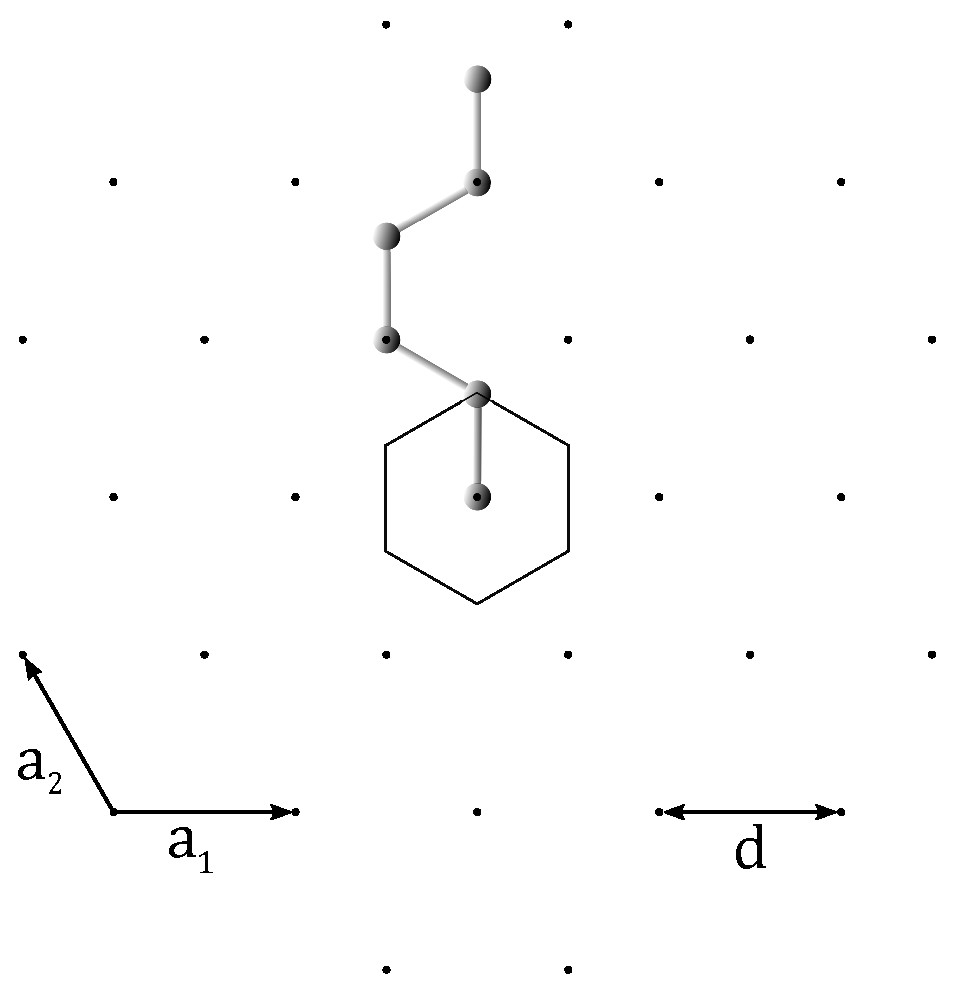
\includegraphics[width=0.5\textwidth]{Figures/hexagon2.eps}
 \caption{Hexagonal Bravais lattice structure with generating vectors $\mathbf{a_{1}}$ \& $\mathbf{a_{2}}$. The Hexagon in the middle with the solid lines is unit cell and the shaded elements are the carbon atoms placed in the lattice.}
 \label{hexagon}
\end{figure}

% !TEX root = ../Main.tex

\subsection{Nanomechanics}
This following section will focus on the mechanics of the now defined geometry of the Graphene sheet. It will incorporate boundary conditions in two dimensions, Hooke's law, the normal modes of the lattice as well as phonons. Most of the ideas, formulas and the workthrough in general, has its roots in the book \text{\cite{Cleland2003}}. We refer the reader to this box for a more detailed describtion of nanomechanics.  
\subsubsection{Mechanics and dynamics of a simple system containing two atoms PLOTS??}
To describe the dynamics of the system one must decompose the system into simpler elements in order to understand what happens for the system as a whole. Basically we want to describe the displacements each atom makes and then sum it up to some bigger form of system. The basis of a system containing only two atoms can be described a mass-spring system where each atom has a mass and where the \textit{atomic interaction potential} works as the spring in between each atom. The specific interaction potential we will be working with is called the \textit{Lennard-Jones Potential}\text{\cite[eq.1.3]{Cleland2003}}. The potential is given by \begin{equation}
    \phi(r)=-\dfrac{A}{r^{6}}+\dfrac{B}{r^{12}}\label{LJPot}
\end{equation} where $A$ is the strength of the attractive interaction , $B$ is the strength of the repulsive interaction and $r$ is the spacing between the atoms.
The potential can be derived from the force between the atoms as the force is the derivative of the negative potential energy with respect to the atom spacing $r$\text{\cite[eq.1.1]{Cleland2003}}.\begin{equation}
    f(r)\equiv -\dfrac{\text{d}\phi}{\text{d}r}
\end{equation} However it is more convenient to work with the potential instead of the force. \\
The system is in a relaxed state when the distance between the atoms is equal to the \textit{equilibrium distance} $r=r_{0}$. The equilibrium distance\text{\cite[p.3]{Cleland2003}} is given by \begin{equation}
    r_{0}=\left(\dfrac{2B}{A}\right)^{\dfrac{1}{6}}\label{eqdist}
\end{equation} Inserting \eqref{eqdist} in \eqref{LJPot} gives the minimum potential energy \begin{equation}
    \phi(r_{0})=-\dfrac{A^{2}}{4B}
\end{equation}When we work with larger systems we want the system to be relaxed i.e. in equilibrium first. However, for such systems it is not always the case hence why it must be relaxed with the required relaxation energy before we can apply external forces on it. Now that the small system has been described in its equilibrium state. We want to know what happens when we displace the atoms from their equilibrium position, that is to exert an external force on the atoms. As it is with all masses within classic mechanical theory, the atoms will start to oscillate around their equilibrium position. Therefore a \textit{harmonic potential approximation} is needed to describe the energy associated with such a displacement. This approximation only works for small displacements from equilibrium i.e. small external forces. This is because the approximation is made by using a \textit{Taylor series} expansion\text{\cite[eq.1.5]{Cleland2003}} where only the first and second order terms are kept hence the approximation fails the further you get away from the equilibrium position. The expansion of the potential is given by
\begin{align}
    & \phi(r)=\phi(r_{0})+\left\dfrac{\text{d}\phi}{\text{d}r} \right|_{r_{0}}(r-r_{0})+\nonumber\\ & \left\dfrac{1}{2!}\dfrac{\text{d}^{2}\phi}{\text{d}r^{2}}\right|_{r_{0}} (r-r_{0})^{2}+\nonumber\\ & \dfrac{1}{3!}\left\dfrac{\text{d}^{3}\phi}{\text{d}r^{3}}\right|_{r_{0}}(r-r_{0})^{3}+...
\end{align}Where the term $\left\dfrac{\text{d}\phi}{\text{d}r} \right|_{r_{0}}$ equals 0 at equilibrium position. Dropping the higher order terms the series becomes the \textit{harmonic potential approximation}\text{\cite[eq.1.5]{Cleland2003}}\begin{equation}
    \phi(r)\approx \phi(r_{0})+\left\dfrac{1}{2}\dfrac{\text{d}^{2}\phi}{\text{d}r^{2}}\right|_{r_{0}}(r-r_{0})^{2}\label{Harmapprox}
\end{equation}It can be seen that the potential energy depends on the displacement from equilibrium squared. When the atoms are in the presence of an external force, that is when they are displaced from equilibrium. The total potential energy\text{\cite[p.4]{Cleland2003}} becomes $U_{tot}=\phi(r)+\phi_{ext}(r)$, where $\phi_{ext}(r)=-f_{ext}r$. When a constant external force acts on the system, the point of equilibrium moves to a new location. At the location, the derivative of the total potential energy with respect to the displacement is zero
$\dfrac{\text{d}U_{tot}}{\text{d}r}=0$. Working on with this expression and using the result in \eqref{Harmapprox} the total energy in the point of the new equilibrium can described as\begin{align}
    & \dfrac{\text{d}U_{tot}}{\text{d}r}=\dfrac{\text{d}\phi(r)}{\text{d}r}+\dfrac{\text{d}\phi_{ext}(r)}{\text{d}r}=0\nonumber\\
    & \dfrac{\text{d}}{\text{d}r}\left(\phi(r_{0})+\dfrac{1}{2}\left\dfrac{\text{d}^{2}\phi(r)}{\text{d}r^{2}}\right|_{r_{0}}(r-r_{0})^{2}\right)-\nonumber\\ & \dfrac{\text{d}}{\text{d}r}f_{ext}r=0\nonumber\\
    &\dfrac{\text{d}}{\text{d}r}\left(\dfrac{1}{2}\left\dfrac{\text{d}^{2}\phi(r)}{\text{d}r^{2}}\right|_{r_{0}}(r-r_{0})^{2}\right)-f_{ext}=0
    \end{align}The square of the displacement gives the three terms $r^{2}-2r_{0}r+r_{0}^{2}$ that only leaves $2r-2r_{0}$ when derived with respect to $r$. This leaves\begin{align}
   & \dfrac{1}{2}\left\dfrac{\text{d}^{2}\phi(r)}{\text{d}r^{2}}\right|_{r_{0}}(2r-2r_{0})-f_{ext} =0\nonumber\\
   & \left\dfrac{\text{d}^{2}\phi(r)}{\text{d}r^{2}}\right|_{r_{0}}(r-r_{0}) =f_{ext}\nonumber\\
   & r-r_{0} =\dfrac{1}{\text{d}^{2}\phi(r)/\text{d}r^{2}}f_{ext}\label{hooke}
    \end{align}If the  displacement is defined as $u\equiv r-r_{0}$ we can see that \eqref{hooke} is an equivalent to Hooke's Law.\begin{equation}
        u\equiv r-r_{0}=\dfrac{1}{\text{d}^{2}\phi(r)/\text{d}r^{2}}f_{ext}=\dfrac{1}{k}f_{ext}
    \end{equation}Where $k=\dfrac{\text{d}^{2}\phi(r)}{\text{d}r^{2}}$ acts as the spring constant. This last result emphasises that the system of two atoms can be viewed as a mass-spring system.\\
    \eqref{hooke} can also be used to find the equation of motion. As the force equals mass times acceleration the equation must satisfy\begin{equation}
        f_{ext}=\left\dfrac{\text{d}^{2}\phi(r)}{\text{d}r^{2}}\right|_{r_{0}}u=ma=m\dfrac{\text{d}^2}{\text{d}t^2}u
    \end{equation}For the specific case of the two atoms the equation becomes\begin{equation}
        \mu \dfrac{\text{d}^2}{\text{d}t^{2}}u=-\left\dfrac{\text{d}^{2}\phi(r)}{\text{d}r^{2}}\right|_{r_{0}}u\label{eqmotion}
    \end{equation}Where $\mu$ is the reduced mass of the two atoms $\dfrac{1}{\mu}=\dfrac{1}{m_{1}}+\dfrac{1}{m_{2}}$ and the sign in front of the right side of \eqref{eqmotion} is indicating that the force is the restoring force opposing the external force $f_{ext}$. The normal mode solution\text{\cite[eq.1.17]{Cleland2003}} to this equation is\begin{equation}
        u(t)=u_{0}\text{cos}(\omega_{0}t+\varphi)=\text{Re}\left(u_{0}e^{-i\omega_{0}t}\right)
    \end{equation} and the resonance frequency $\omega_{0}$\text{\cite[eq.1.18]{Cleland2003}} is given by\begin{equation}
        \omega_{0}=\sqrt{\dfrac{1}{\mu}\dfrac{\text{d}^2\phi}{\text{d}r^{2}}}=\sqrt{\dfrac{k}{\mu}}
    \end{equation} This concludes the example of a system of two atoms. 
    The next step is to scale up this theory to two and three dimensions.
\subsubsection{Dynamics in a three dimensional lattice} As we have now moved on to three dimensions the position of each atom now has three coordinates and we will be working with bulk systems containing many atoms. To accommodate for these changes we will use vector notation. Otherwise the progression will be similar to the two atom system, first defining the interaction potential with the harmonic approximation and a \textit{Tensor} function, then the system of equations of motion which contains a \textit{Dynamical Matrix}, an eigenvector-eigenvalue problem as well as the wavevector $\textbf{q}$ and at last discussing the solutions to the system of equations.\\
To describe the atoms in the lattice and their vector field displacement $\mathbf{u}(\mathbf{r},t)$ we are still going to use classic mechanical theory as every atom in the lattice are seen as point masses, just like the system of two atoms. As defined in \cref{BLGV} we have a lattice with $\mathbf{R}_{j}$ lattice points. In \cref{BLGV} we look at a two dimensional lattice but the following will describe a three dimensional lattice which basically means that $\mathbf{R}_{j}$ will have an additional coordinate. As it was with the system of two atoms, we want this system to be at equilibrium and therefore we choose an origin where the atom at the center of the $j$'th unitcell is placed on the $\mathbf{R}_{j}$ lattice point. Again looking at \cref{hexagon} that would be an example of such as system in two dimensions. A continuous displacement of the whole lattice $\mathbf{u}(\mathbf{r},t)$ is now added to the lattice. The displacement is defined at every point $\mathbf{r}$ in the lattice which means that it is also defined in between the lattice points $\mathbf{R}_{j}$. The use of such displacement implicates that the atoms in the $j$'th unitcell will be displaced\text{\cite[p.57]{Cleland2003}} by $\mathbf{r}_{j}=\mathbf{R}_{j}+\mathbf{u}(\mathbf{r}_{j},t)$. Again we are going to employ a harmonic approximation for the system and for that to be successful, one have to assume very small displacements, i.e. very mall $\mathbf{u}$. Because of the assumption of very small displacements, the displacement field will be evaluated at the equilibrium position $\mathbf{R}_{j}$ instead of the instantaneous position $\mathbf{r}_{j}$. The displacement function can therefore be described as $\mathbf{u}(\mathbf{r}_{j},t)\approx \mathbf{u}(\mathbf{R}_{j},t)$. With displacement defined we can describe where the $j$'th atom is located at time $t$: $\mathbf{r}_{j}=\mathbf{R}_{j}+\mathbf{u}(\mathbf{R}_{j},t)\rightarrow \mathbf{r}_{j}=\mathbf{R}_{j}+\mathbf{u}_{j}(t)$ using $\mathbf{u}_{j}(t)=\mathbf{u}(\mathbf{R}_{j},t)$ as a short hand. As with the system of two atoms, the interaction potential energy of a two or three dimensional system is dependent on some displacement from equilibrium, why the total potential energy can be described with a function containing all atoms positions at a time $t$. The potential energy takes the form $U=U(\mathbf{r}_{1},\mathbf{r}_{2},\mathbf{r}_{3},...\mathbf{r}_{N})$. Now that we have function for the total potential energy, using a small displacement $\mathbf{u}_{j}(t)$, the harmonic approximation can be written up using a Taylor expansion\text{\cite[eq.2.29]{Cleland2003}}.\begin{align}
   & U(\mathbf{r}_{1},\mathbf{r}_{2},...\mathbf{r}_{N})= \nonumber\\
    & U(\mathbf{R}_{1},\mathbf{R}_{2},...\mathbf{R}_{N})+\sum_{j=1}^{N}\sum_{\alpha=1}^{3}\left\dfrac{\partial U}{\partial r_{j\alpha}}\right|_{\mathbf{R}_{j}}u_{j\alpha}+\nonumber\\
    & \sum_{j,k=1}^{N}\sum_{\alpha,\beta=1}^{3}\dfrac{1}{2}\left\dfrac{\partial^{2} U}{\partial r_{j\alpha}\partial r_{k\beta}}\right|_{\mathbf{R}_{j}}u_{j\alpha}u_{k\beta}+...
\end{align}Just like the two atom system the second term\begin{equation*}
    \sum_{j,k=1}^{N}\sum_{\alpha=1}^{3}\left\dfrac{\partial U}{\partial r_{j\alpha}}\right|_{\mathbf{R}_{j}}u_{j\alpha}=0
\end{equation*} at equilibrium, moreover the potential energy at the equilibrium positions $\mathbf{R}_{j}$ also equals 0. Again, dropping the higher order terms, this leaves us with the harmonic approximation\text{\cite[eq.2.30]{Cleland2003}}\begin{align}
    & U_{harm}(\mathbf{r}_{1},...\mathbf{r}_{N})=\nonumber\\ & \dfrac{1}{2}\sum_{jk=1}^{N}\sum_{\alpha\beta=1}^{3}\left\dfrac{\partial^{2} U}{\partial r_{j\alpha}\partial r_{k\beta}}\right|_{\mathbf{R}_{j}}u_{j\alpha}u_{k\beta}\label{harmapprox2}
\end{align}In order to simplify the notation when working with the dynamics of the system, we introduce a \textit{tensor}\text{\cite[p.58]{Cleland2003}} which is a $3x3$ matrix. The tensor does not change when translated to another coordinate system, but elements within the tensor does change however. The tensor\text{\cite[eq.2.31]{Cleland2003}} is defined by\begin{equation}
    \Phi_{\alpha\beta}(\mathbf{R}_{i},\mathbf{R}_{j})=\left\dfrac{\partial^{2}U}{\partial r_{i\alpha}\partial r_{j\beta}}\right|_{\mathbf{R}_{j}} 
\end{equation} and is in terms of the curvature of the total interaction energy $U(\mathbf{r}_{1},...\mathbf{r}_{N})$\text{\cite[p.58]{Cleland2003}}. As the tensor are only dependent on the equilibrium positions $\mathbf{R}_{i},\mathbf{R}_{j}$ the crystal itself does not change under translation. This means that the tensor only depend on the difference in the atoms poitions. The tensor then becomes\text{\cite[eq.2.32]{Cleland2003}}\begin{equation}\Phi_{\alpha\beta}(\mathbf{R}_{i},\mathbf{R}_{j})=\Phi_{\alpha\beta}(\mathbf{R}_{i}-\mathbf{R}_{j})
\end{equation}This will also change \cref{harmapprox2} to\begin{align}
    &U_{harm}(\mathbf{r}_{1},...\mathbf{r}_{N})=\nonumber\\
    &\dfrac{1}{2}\sum_{jk=1}^{N}\sum_{\alpha\beta=1}^{3}u_{j\alpha}\Phi_{\alpha\beta}(\mathbf{R}_{j}-\mathbf{R}_{k})u_{k\beta}
\end{align}. Now that an expression for the total potential energy has been described, we need an expression for total kinetic energy in order to write of the Hamiltonian for the system. As we have already described the displacement of the system with the displacement field $\mathbf{u}_{j}$, the kinectic energy\text{\cite[eq.2.28]{Cleland2003}} for the system is pretty straight forward.\begin{equation}
    T=\dfrac{1}{2}M\sum_{j=1}^{N}\left|\dfrac{\partial\mathbf{u}_{j}}{\partial t}\right|^{2}
\end{equation}The Hamiltonian\text{\cite[eq.2.44]{Cleland2003}} for system becomes\begin{align}
    & H=\dfrac{1}{2}M\sum_{j=1}^{N}\left|\dfrac{\partial\mathbf{u}_{j}}{\partial t}\right|^{2}+\nonumber\\
    & \dfrac{1}{2}\sum_{jk=1}^{N}\sum_{\alpha\beta=1}^{3}u_{j\alpha}\Phi_{\alpha\beta}(\mathbf{R}_{j}-\mathbf{R}_{k})u_{k\beta}
\end{align}. The equation of motion for the system can be derived by setting the Hamiltonian equal to 0.\begin{align}
    & \dfrac{1}{2}M\sum_{j=1}^{N}\left|\dfrac{\partial\mathbf{u}_{j}}{\partial t}\right|^{2}+\nonumber\\
    & \dfrac{1}{2}\sum_{jk=1}^{N}\sum_{\alpha\beta=1}^{3}u_{j\alpha}\Phi_{\alpha\beta}(\mathbf{R}_{j}-\mathbf{R}_{k})u_{k\beta}=0\label{hamil}
\end{align} Taking every index of $\alpha$, the displacement vector becomes $\mathbf{u}_{j}=u_{\alpha j}$. Moving things around in \cref{hamil} we get\begin{align}
     & \dfrac{1}{2}M\sum_{\alpha=1}^{3}\sum_{j=1}^{N}\dfrac{\partial^{2}}{\partial t^{2}}u_{j\alpha}^{2}=\nonumber\\
    & -\dfrac{1}{2}\sum_{jk=1}^{N}\sum_{\alpha\beta=1}^{3}u_{j\alpha}\Phi_{\alpha\beta}(\mathbf{R}_{j}-\mathbf{R}_{k})u_{k\beta}\\
    & M\dfrac{\partial^{2}}{\partial t^{2}}u_{j\alpha}=-\sum_{k=1}^{N}\sum_{\beta=1}^{3}\Phi_{\alpha\beta}(\mathbf{R}_{j}-\mathbf{R}_{k})u_{k\beta}
\end{align}Solving this system of equations requires finding the normal modes for system which is the same as the general solution for the system of equations. This means that all solutions must have the same time dependence. As the general solution form a complete set, we can describe the any motion in the lattice as a superposition of normal modes. When we take the same time dependence for all atoms in the lattice we get the same solution as with the two atom system, just in vector notation.\begin{equation}
    \mathbf{u}_{j}(t)=\mathbf{A}_{j}e^{i\omega t}
\end{equation}Here $\mathbf{A}_{j}$ is the displacement for the $j$'th atom in all three directions. 


\subsubsection{Periodic functions}
\subsubsection{Reciprocal space, Blochs theorem, Bloch wavevector}

\subsubsection{Boundary Conditions in Two Dimensions}

When describing the motion of the atoms in the lattice as well as the forces acting upon them, some boundary conditions must be defined. Because the system is very large compared to the characteristic wavelength in the displacement field, periodic boundary conditions (PBC) work well. The actual boundaries as well as the specific normal modes are not of significant importance due the same fact of size difference in the system vs. the characteristic wavelength. \\
An intuitive approach to imagining PBC is to take the plane of the system and fold it in to at torus. All the four edges has now been put together pairwise. This means that any force acting on one atom which causes some form of motion is now translated on to the atom next to it.\\
For an arbitrary system in two dimensions of size $X$ (side lenght) and with atomic spacing $r_{0}$, each axis has $\mathcal{N}=\dfrac{X}{r_{0}}$ atoms. The total amount of atoms in the sheet naturally becomes $N=\mathcal{N}^{2}$. The Bloch wavevector can be described as
\begin{equation}
     \mathbf{q}=(q_{x},q_{y})
\end{equation}
where
\begin{equation}
     (q_{x},q_{y})=\dfrac{2\pi}{X}(m,n)
\end{equation}
Here $m,n$ are integers in the interval $-\dfrac{\mathcal{N}}{2}, +\dfrac{\mathcal{N}}{2}$. The range of $q_{x},q_{y}$ becomes $-\dfrac{\pi}{r_{0}},+\dfrac{\pi}{r_{0}}$.\\
In the specific case of this study we work with a fixed boundary, more specific, a clamped boundary which means that no bending is allowed in the plane. A clamped boundary results in the need for numerical approximations in calculations of the dynamics. As the tools used for calculations are on a"per atom" atom basis, there wont be any need for finite-element models nor any partial differential equations solver (PDE). Instead...

\subsubsection{Normal Modes of Two-Dimensional Hexagonal lattice}
 

% !TEX root = ../Main.tex

% !TEX root = ../Main.tex

\subsection{Atomistix ToolKit: ATKPython and Nanolanguage}
In this project we will utilise the Atomistix ToolKit, developed by QuantumWise\footnote{QuantumWise' webpage: \href{https://quantumwise.com/}{https://quantumwise.com/}}, or ATK for short. The Toolkit takes Python scripts as inputs and simulates a completely custom lattice enviroment with various applied calculations. It is possible to simulate very specific scenarios, alter the simulation parameters and extract results for analysis easily and fast.
ATKPython (the standalone simulation program) extends the Python language with Nanolanguage which tells ATKPython what to do when launched. One can set up specific bravais lattices and repeat them into large 2D structures. Then specific atoms can be tagged or altered and calculations can be set up. All of these features are available through QuantumWise VNL, a GUI which sets up the scripts and calculations, if need be. The GUI is shown on \cref{VNLLAB}. When working with VNL both GUI and CLI are used. The GUI can be used to setup the simulation and the simulation files can be altered to eg. producing custom datasets. The typical workflow when using VNL and ATK is depicted on \cref{workflow}
\begin{figure}
 \centering
 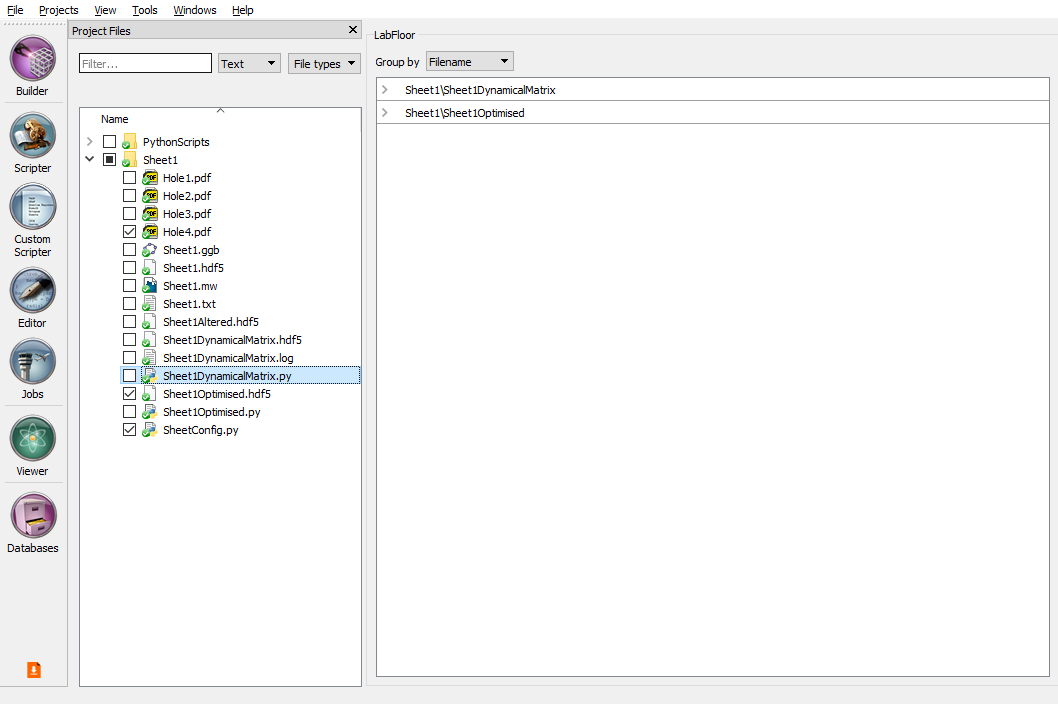
\includegraphics[width=\columnwidth]{Figures/VNLLabfloor.png}
 \caption{The VNL Labfloor user interface shows project files in the center frame and various tools in the left pane.}
 \label{VNLLAB}
\end{figure}
\begin{figure}
  \centering
  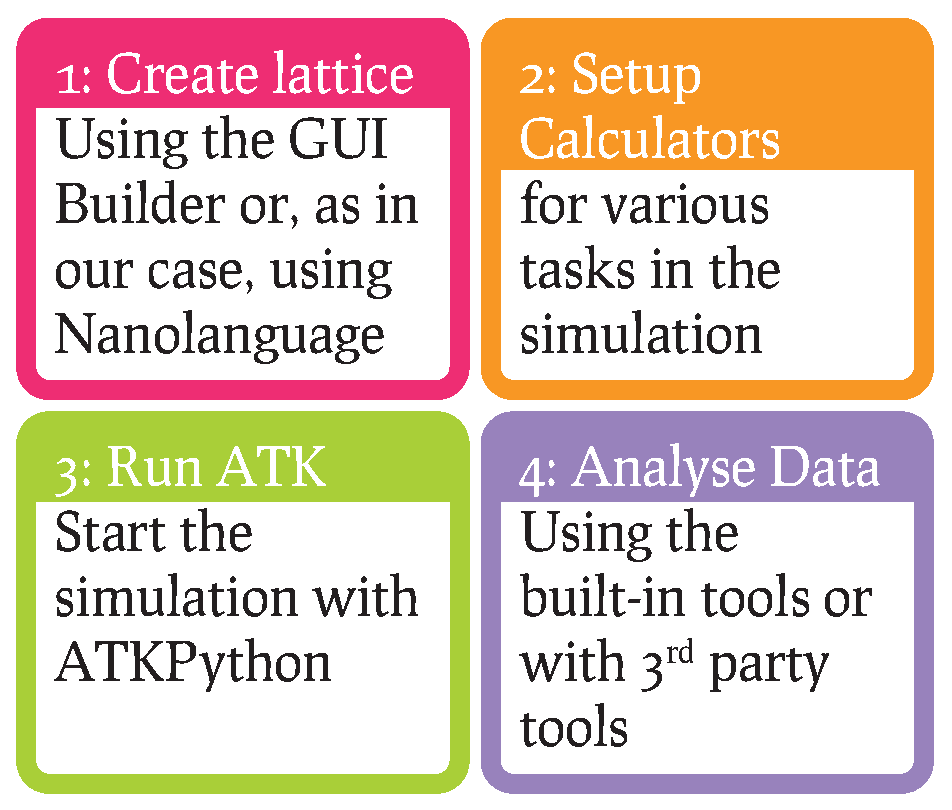
\includegraphics[width=\columnwidth]{Figures/Workflow.eps}
  \caption{Diagram showing the typical workflow in VNL.}
  \label{workflow}
\end{figure}

%End of text

%Bibliography herunder:
\newpage

\bibliography{Physics-Project-Nanomechanics-for-Graphene-Membranes}

\newpage
\listoffigures
\listoftables
\listoflistings
\onecolumngrid
\newpage
%Appendicer herunder:
% !TEX root = Main.tex

\appendix
\appendixpage
\addappheadtotoc
%\section{Animation of \nth{9} mode}
%\begin{center}
%  \animategraphics[autoplay,loop,width=\textwidth]{60}{VNL/Frames/frame}{1}{60}
%\end{center}
%Section 1 herunder:
\section{NanoSheetCreator.py}
\label{NSCstart}
\inputminted[python3=true,bgcolor=Black,linenos=true]{python}{VNL/PythonScripts/NanoSheetCreator.py}
\label{NSCend}
%Section 2 herunder:
\todo[inline]{Correct graph}
\begin{figure}
  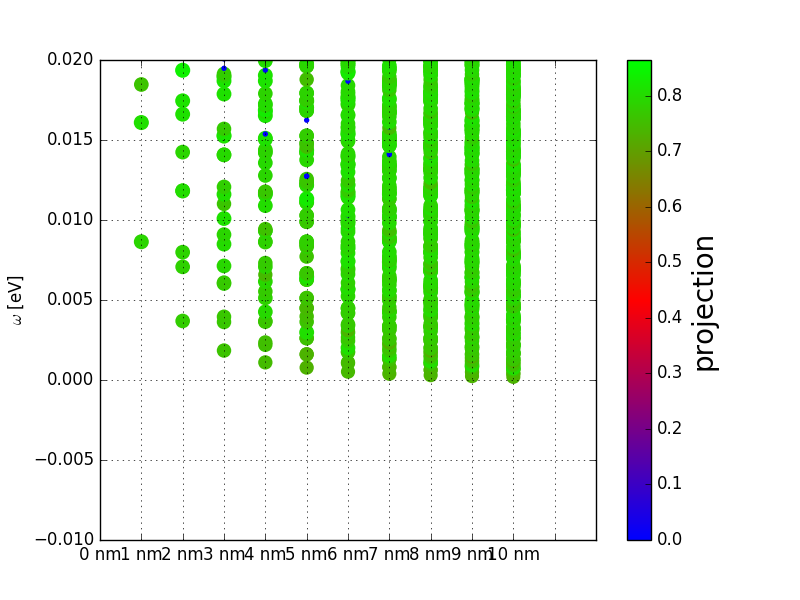
\includegraphics[width=\textwidth]{VNL/PythonScripts/FrequencyVSSize/PlottingArea/FrequencyModeProjections.eps}
  \caption{$\omega(r)$}
  \label{OR}
\end{figure}
\newpage

\end{document}
